\documentclass{beamer}
\usepackage{etex}

\usepackage[utf8]{inputenc}
\usepackage[frenchb]{babel}
\usepackage{verbatim}
\usepackage{graphicx}
\usepackage{color}
\usepackage{hyperref}
\usepackage{verbatim}
\usepackage{url}
\usepackage{moreverb}
\usepackage{fancyvrb}
\usepackage{minted}
\usepackage{natbib}
\usepackage{eulervm}
\usepackage{auto-pst-pdf}
\usepackage{pst-plot}
\usepackage{amssymb}% http://ctan.org/pkg/amssymb
\usepackage{pifont}% http://ctan.org/pkg/pifont
\usepackage{tikz}
\newcommand{\cmark}{\ding{51}}%
\newcommand{\xmark}{\ding{55}}%

\usetikzlibrary{shapes,arrows}
\tikzset{
  every overlay node/.style={
    draw=white,fill=white,anchor=north west,
  },
  every overlay node border/.style={
    draw=black,fill=white,anchor=north west,rounded corners,
  },
}
% Usage:
% \tikzoverlay at (-1cm,-5cm) {content};
% or
% \tikzoverlay[text width=5cm] at (-1cm,-5cm) {content};
\def\tikzoverlay{%
   \tikz[baseline,overlay]\node[every overlay node]
}%
\def\tikzoverlayborder{%
   \tikz[baseline,overlay]\node[every overlay node border]
}%

\newrgbcolor{mygreen}{.00 .5 .00}
\newcommand{\X}[1]{\textcolor{blue}{#1}}
\newcommand{\y}[1]{\textcolor{red}{#1}}
\newcommand{\model}[1]{\textcolor{mygreen}{#1}}
\newcommand{\loss}[1]{\textcolor{lightblue}{#1}}

\hypersetup{colorlinks=true, linkcolor=black, urlcolor=blue}
\usetheme{boxes}
\beamertemplatenavigationsymbolsempty
\setbeamertemplate{sections/subsections in toc}[circle]
\setbeamertemplate{footline}[frame number]
\setbeamertemplate{itemize items}[circle]
\setbeamertemplate{itemize subitem}[square]

\title{\bf Ethnicity Sensitive Author Disambiguation Using Semi-supervised Learning}
\author{Gilles Louppe, Hussein Al-Natsheh, Mateusz Susik \\and 
Eamonn Maguire}
\institute{KESW 2016, Prague}
\date{September 23, 2016}

\newcommand{\todo}[1]{\textcolor{red}{[TODO] #1}}

\DeclareMathOperator*{\argmax}{arg\,max}

\begin{document}

\begin{frame}
\titlepage
\end{frame}


% Motivation ==================================================================

\begin{frame}{Motivation}
For each author, group together all his publications, and only those.

\footnotesize{
\begin{columns}[T]

\begin{column}{0.33\textwidth}
\begin{figure}
\texttt{M.S.Smith.1}
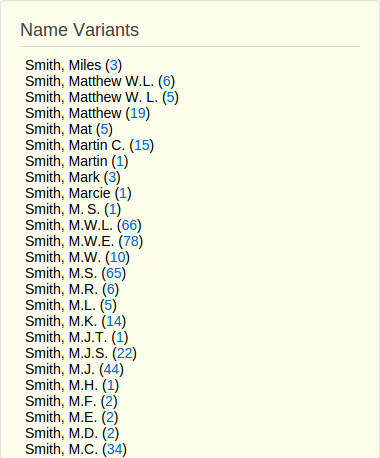
\includegraphics[width=\textwidth]{figures/no-more.png}
\end{figure}
\end{column}
\begin{column}{0.33\textwidth}
\begin{figure}
\texttt{Z.Liang.4}
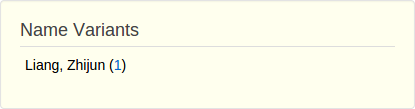
\includegraphics[width=\textwidth]{figures/no-less.png}

\texttt{Z.Liang.5}
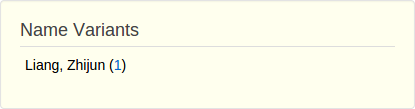
\includegraphics[width=\textwidth]{figures/no-less.png}

...

\texttt{Z.Liang.83}
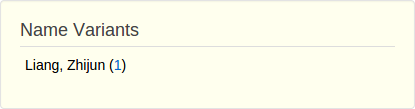
\includegraphics[width=\textwidth]{figures/no-less.png}
\end{figure}
\end{column}
\begin{column}{0.33\textwidth}
\begin{figure}
\texttt{S.W.Hawking.1}
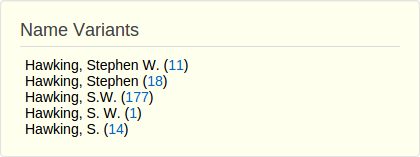
\includegraphics[width=\textwidth]{figures/exact.png}
\end{figure}
\end{column}

\end{columns}

\begin{columns}[T]
\begin{column}{0.33\textwidth}
\begin{center}{\it No more}\end{center}
\end{column}
\begin{column}{0.33\textwidth}
\begin{center}{\it No less}\end{center}
\end{column}
\begin{column}{0.33\textwidth}
\begin{center}{\it But all and only the correct ones}\end{center}
\end{column}
\end{columns}}
\end{frame}

\begin{frame}

\tikzstyle{block} = [rectangle, draw, text width=10em, text centered, rounded corners, minimum height=2em]
\tikzstyle{line} = [draw, -latex']
\tikzstyle{cloud} = []

\begin{center}
\begin{tikzpicture}[node distance = 2cm, auto]
    % Place nodes
    \node [block] (clustering) {Author disambiguation};
    \node [cloud, above of=clustering] (input1) {$\{s_1, s_2, ..., s_N\}$};
    \node [cloud, below of=clustering] (output) {$\{ \underbrace{\{ s_1, s_3, s_4 \}}_{\text{author 1}}, \underbrace{\{ s_2, s_5\}}_{\text{author 2}}, ... \}$};
    % Draw edges
    \path [line] (input1) -- (clustering);
    \path [line] (clustering) -- (output);
\end{tikzpicture}
\end{center}
\end{frame}



% Spread of the problem =======================================================

\begin{frame}{Spread of the problem}

As extracted from claimed publications in INSPIRE,

\begin{itemize}
\item {\color{blue} Authors have on average $2.06$ name variants (synonyms)}\\
Eg.: Doe, John; Doe, J.
\item {\color{blue} Unique name variants are shared on average by $1.04$ authors (homonyms)}
\end{itemize}

Clustering on exact full names or last name + first initial, should
yield very good results on average.

\vskip1em

{\color{red} But}, disambiguation issues are expected to amplify with the rise of Asian researchers:
Caucasian names (now representative of INSPIRE authors) are almost never
ambiguous, while Asian names are very often.

% compute average number of name variants per author (synonyms)
% compute average number of authors per name variants
% => easy but we want to do better

\end{frame}


% How would you fare? =========================================================

\begin{frame}{How would \textit{you} fare?}

\only<1-2>{
\begin{figure}
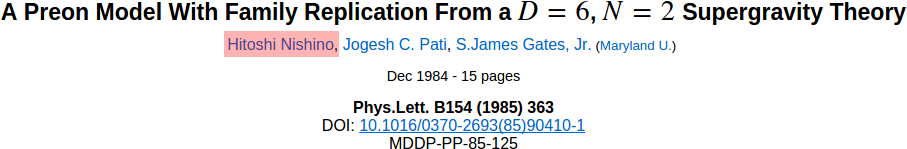
\includegraphics[scale=0.35]{figures/author1/1.png}\\[2em]
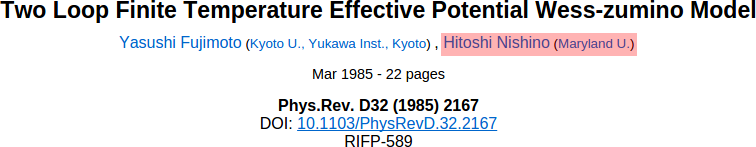
\includegraphics[scale=0.35]{figures/author1/2.png}\\[2em]
\uncover<2>{\color{blue} \cmark~ Same authors}
\end{figure}
}
\only<3-4>{
\begin{figure}
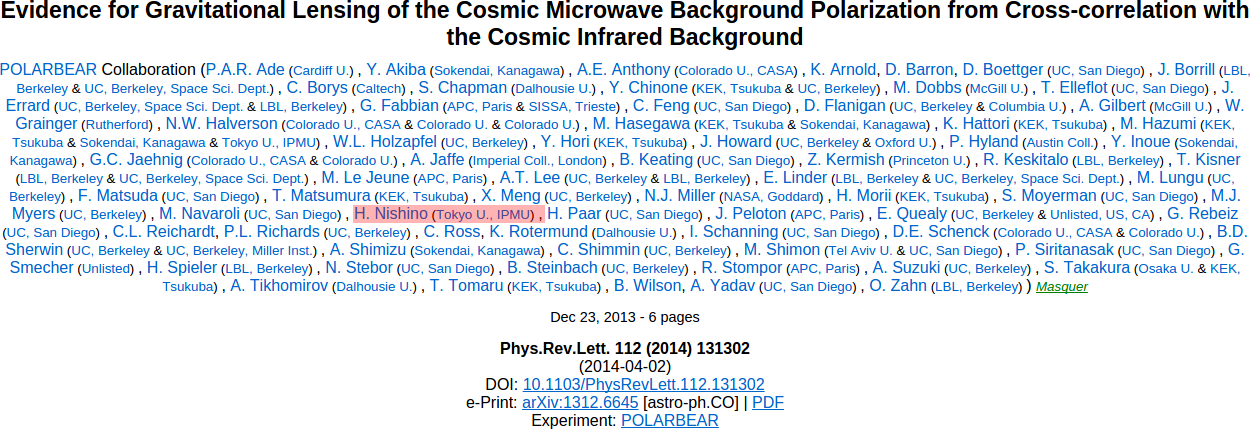
\includegraphics[scale=0.25]{figures/author2/3.png}\\[2em]
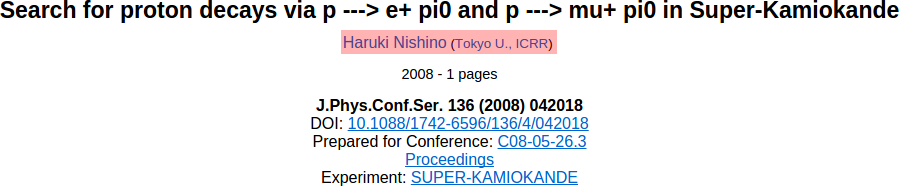
\includegraphics[scale=0.35]{figures/author2/1.png}\\[1em]
\uncover<4>{\color{blue} \cmark~ Same authors}
\end{figure}
}
% \only<5-6>{
% \begin{figure}
% 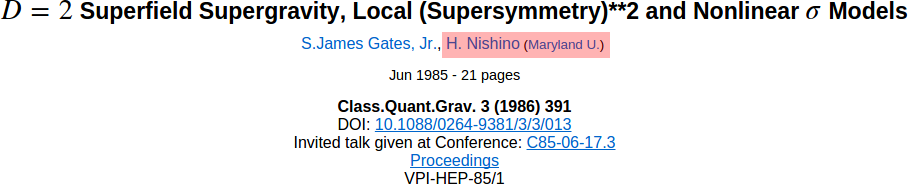
\includegraphics[scale=0.35]{figures/author1/5.png}\\[2em]
% 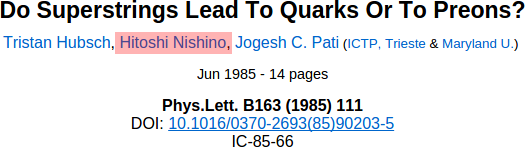
\includegraphics[scale=0.35]{figures/author1/4.png}\\[2em]
% \uncover<6>{\color{blue} \cmark~ Same authors}
% \end{figure}
% }
\only<5-6>{
\begin{figure}
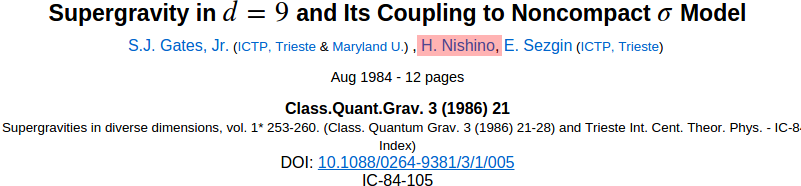
\includegraphics[scale=0.35]{figures/author1/6.png}\\[2em]
\hspace*{-2cm}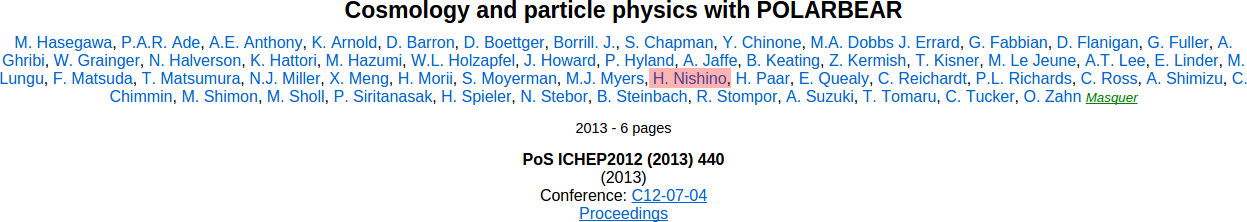
\includegraphics[scale=0.35]{figures/author2/2.png}\\[2em]
\uncover<6>{\color{red} \xmark~ Different authors}
\end{figure}
}
\only<7-8>{
\begin{figure}

\includegraphics[scale=0.35]{figures/author1/3.png}\\[2em]
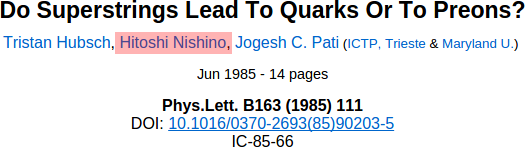
\includegraphics[scale=0.35]{figures/author1/4.png}\\[2em]
\uncover<8>{\color{blue} \cmark~ Same authors}
\end{figure}
}

\end{frame}


% Learning ====================================================================

\begin{frame}{Learning from data}

\begin{itemize}
\item Manual disambiguation is {\color{red} long and difficult}, even for experienced curators.\\[2em]
\item Couldn't we {\color{blue} automatically find a set of rules} to disambiguate two signatures?

$$\varphi(s_1, s_2) = \begin{cases}
    0 & \text{if $s_1$ and $s_2$ belong to the same author},\\
    1 & \text{otherwise}.
  \end{cases}$$

\item This is a machine learning task called {\color{red}supervised learning}.
\end{itemize}

\end{frame}


% Supervised learning =========================================================

\begin{frame}{Supervised learning}

\begin{itemize}
\item The \X{inputs} are random variables \X{$X = X_1$, ..., $X_p$};
\item The \y{output} is a random variable \y{$Y$}.
\end{itemize}

\begin{itemize}
\item Data comes as a finite learning set $${\cal L} = \{(\X{\mathbf{x}_i}, \y{y_i}) | i = 0, \dots, N-1 \},$$
where \X{$\mathbf{x}_i \in {\cal X} = {\cal X}_1 \times ... \times {\cal X}_p$} and \y{$y_i \in {\cal Y}$}
are randomly drawn from $P_{\X{X},\y{Y}}$.\\
\vspace{0.3cm}
\small{
E.g.,:\\
$(\X{\mathbf{x}_i}, \y{y_i}) = ((\X{\text{name sim.}=0.7, \X{\text{title sim.}=0.3}, ...)}, \y{\text{same authors}})$ \\
$(\X{\mathbf{x}_j}, \y{y_j}) = ((\X{\text{name sim.}=0.1, \X{\text{title sim.}=0.5}, ...)}, \y{\text{different authors}})$
}
\end{itemize}

\begin{itemize}
\item The goal is to find a model $\model{\varphi_{\cal L}}: \X{{\cal X}} \mapsto \y{{\cal Y}}$ minimizing
$$
Err(\model{\varphi_{\cal L}}) = \mathbb{E}_{\X{X}, \y{Y}}\{ L(\y{Y}, \model{\varphi_{\cal L}}(\X{X})) \}.
$$
\end{itemize}

\end{frame}



% Publication to Signature ====================================================================

\begin{frame} {Publication to Signature}

\begin{figure}
   \centering
   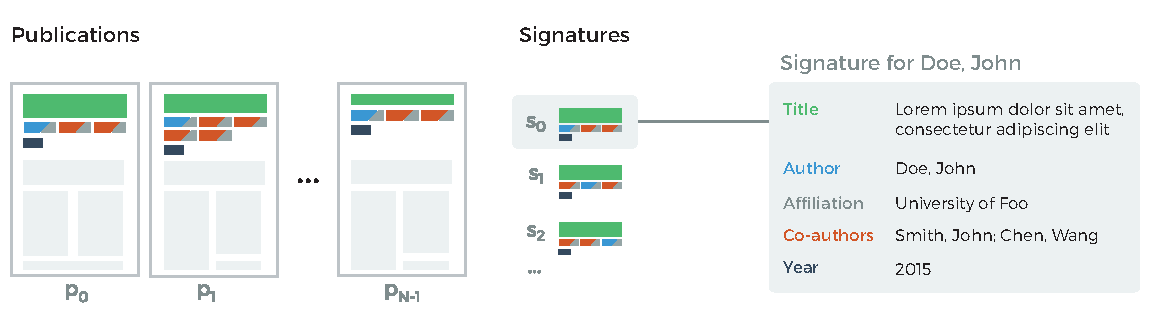
\includegraphics[width=\textwidth]{./figures/fig-pub-to-signature.pdf}
\end{figure}

\end{frame}

% Pipeline ====================================================================

\begin{frame} {General Pipeline}

\begin{figure}
   \centering
   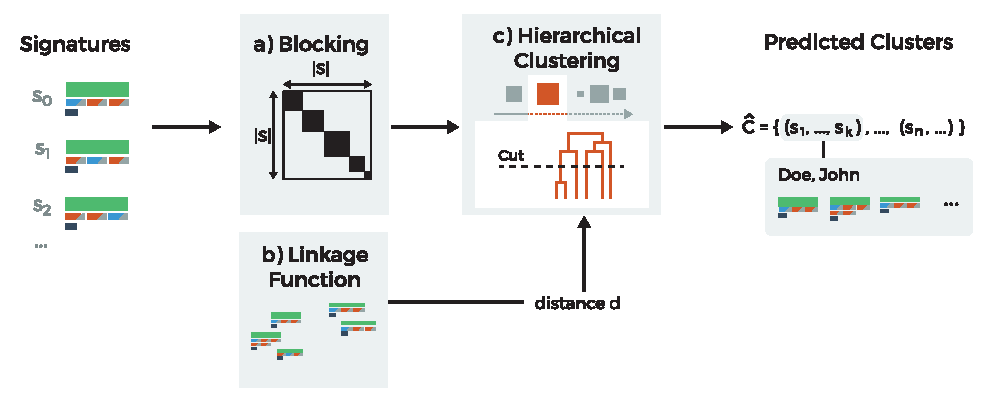
\includegraphics[width=\textwidth]{./figures/fig-workflow.pdf}
\end{figure}

\end{frame}


% GBRT ====================================================================

\begin{frame}{Gradient Boosted Regression Trees [J. Friedman, 1999]}

\begin{itemize}
\item Ensemble of regression trees approximating the (negative) gradient of a loss function
\item Each tree is a successive gradient descent step
\item Low bias and low variance
\end{itemize}


\begin{figure}
   \centering
   \includegraphics[width=\textwidth]{./figures/residual_fitting_2.pdf}
\end{figure}

\tikzoverlay[text width=10cm] at (-0.2cm, 0.1cm) {
\begin{columns}[c]
\begin{column}{0.2\textwidth}
    \begin{figure}
      
\includegraphics[width=2em]{./figures/scikit-learn-logo-thumb.png}
    \end{figure}
\end{column}
\begin{column}{1.0\textwidth}
    \vspace{-0.5cm}\hspace{-0.5cm}{\footnotesize \texttt{sklearn.ensemble.GradientBoostingClassifier|Regressor}}
\end{column}
\end{columns}
};
\end{frame}

% Pair-wise Features Extraction ========================================================

\begin{frame}{Pair-wise Features Extraction}

\begin{figure}
   \centering
   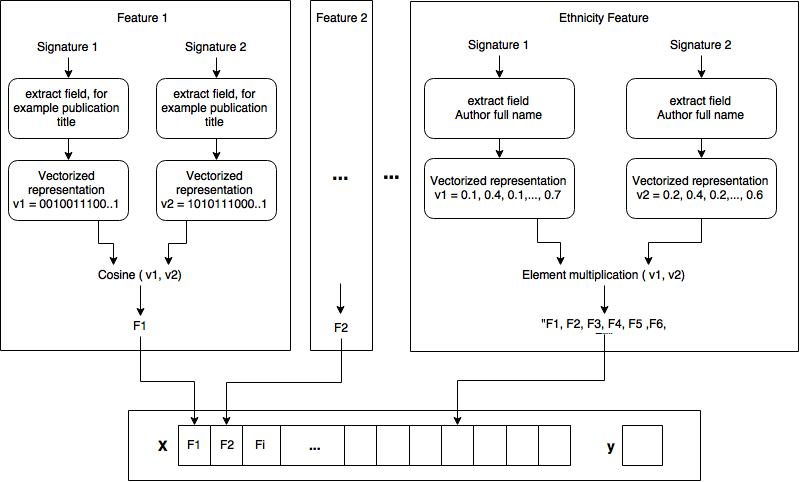
\includegraphics[width=\textwidth]{./figures/pairwise_features.png}
\end{figure}

\end{frame}


% Feature Selection by Recursive Elimination ========================================================

\begin{frame}{Feature Selection by Recursive Elimination}

\begin{figure}
   \centering
   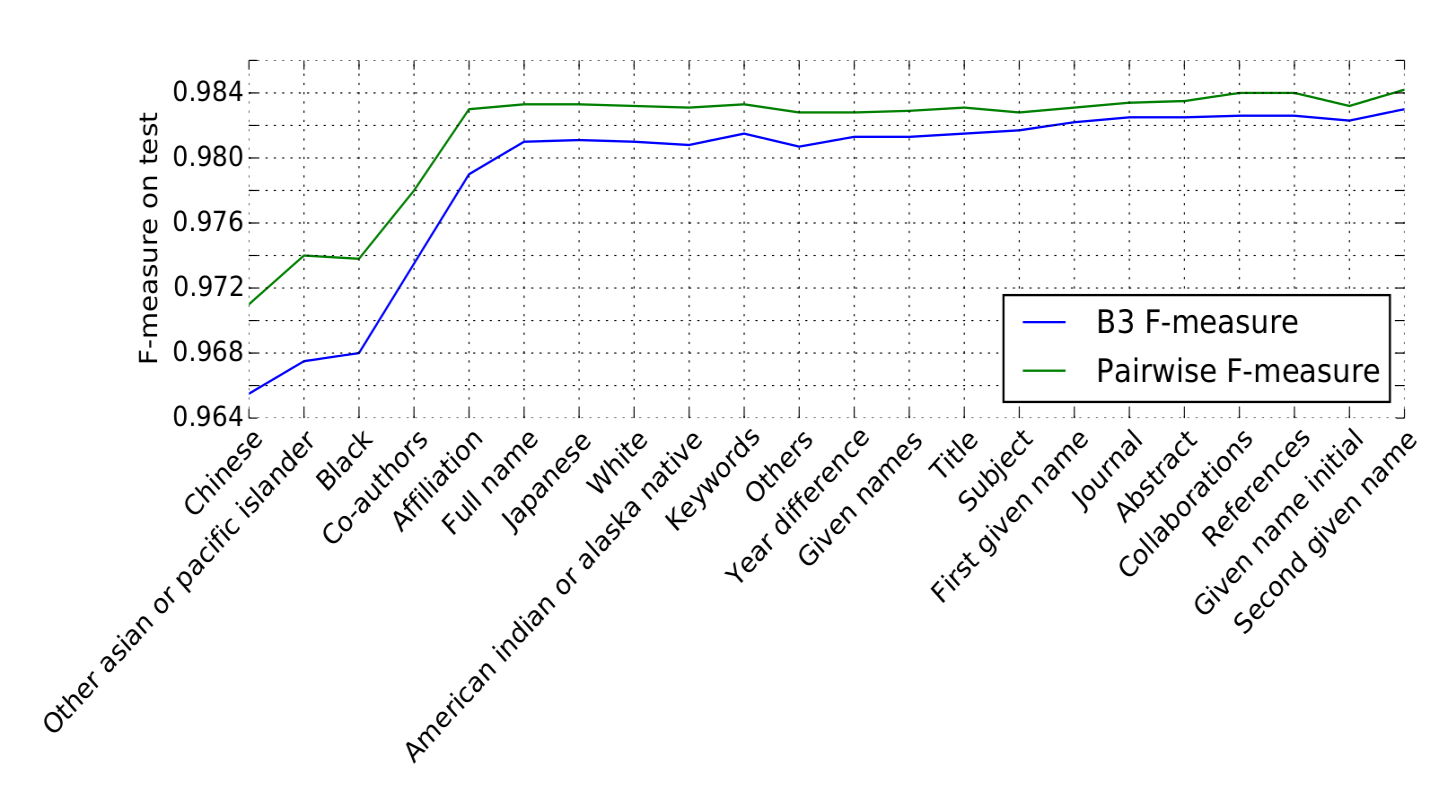
\includegraphics[width=\textwidth]{./figures/fig-rfe.pdf}
\end{figure}

\end{frame}


% Clustering ==================================================================

\begin{frame}{Disambiguation as a Clustering Problem}

\begin{itemize}
\item Author disambiguation = {\color{red} clustering signatures that belong to the same author}.\\[1em]

\item Using our model $\model{\varphi}$, the probability
      that two signatures belong to different authors can be used as a (pseudo) distance metric.
\end{itemize}

\tikzstyle{block} = [rectangle, draw, text width=5em, text centered, rounded corners, minimum height=2em]
\tikzstyle{line} = [draw, -latex']
\tikzstyle{cloud} = []

\begin{center}
\begin{tikzpicture}[node distance = 2cm, auto]
    % Place nodes
    \node [block] (clustering) {Hierarchical clustering};
    \node [cloud, above of=clustering] (input1) {$\{s_1, s_2, ..., s_N\}$};
    \node [cloud, left of=clustering] (input2) {$\varphi$};
    \node [cloud, below of=clustering] (output) {$\{ \underbrace{\{ s_1, s_3, s_4 \}}_{\text{author 1}}, \underbrace{\{ s_2, s_5\}}_{\text{author 2}}, ... \}$};
    % Draw edges
    \path [line] (input1) -- (clustering);
    \path [line] (input2) -- (clustering);
    \path [line] (clustering) -- (output);
\end{tikzpicture}
\end{center}

\end{frame}


% Hierarchical clustering =====================================================

\begin{frame}{Hierarchical Clustering}

\begin{columns}[T]

\begin{column}{0.33\textwidth}
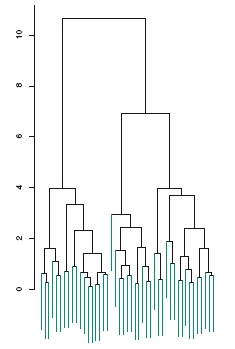
\includegraphics[scale=0.75]{./figures/hierarchy.png}
\end{column}
\begin{column}{0.66\textwidth}
\begin{itemize}
\item General family of clustering algorithms that {\color{blue}build nested clusters by merging them successively}.\\[2em]

\item This hierarchy of clusters is represented as a tree (or dendrogram).\\[2em]

\item The root of the tree is the unique cluster that gathers all the samples, the leaves being the clusters with only one sample.
\end{itemize}
\end{column}

\end{columns}

\end{frame}


% Implementation issues =====================================================

\begin{frame}{Issues}

\begin{itemize}
\item The complexity of hierarchical clustering is {\color{red} $O(N^2)$}. For $N=10^7$ signatures, this is impractical.

{\it Solution:} pre-cluster into blocks all signatures with the same last name + first initial, then cluster each of these blocks.\\[2em]

\item How do you set the {\color{red} cut-off threshold}?

{\it Solution:} using training data (e.g., claimed signatures), pick the threshold that locally maximizes some criterion.
\end{itemize}

\end{frame}

% Partitioning into Blocks =====================================================

\begin{frame} {Solving Issue 1: Partitioning into Blocks}

Talking about blocking goes here (photanic, LNFI...) or in a seperate slide

\begin{columns}[T]

\begin{column}{0.5\textwidth}
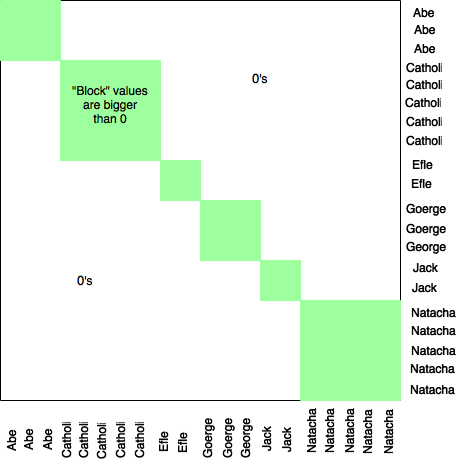
\includegraphics[width=\textwidth]{./figures/blocking.png}
\end{column}
\begin{column}{0.5\textwidth}

Without bloking, the clustering algorithm would deal with:
\begin{itemize}
\item more than $1.07$  million publications.

\item more than $9.27$ millions signatures.

\item more than $1.2$ million claimed signatures (Ground-truth).
\end{itemize}

With blocking, we, somehow, linearize the complexity

\end{column}

\end{columns}

\end{frame}

% Blocking Strategies =====================================================


\begin{frame} {Blocking Strategies}

Talking about blocking goes here (photanic, LNFI...)

\end{frame}


% Cutting Strategy =====================================================


\begin{frame} {Solving Issue 2: Threshold Cut_off Strategy}

\begin{figure}
   \centering
   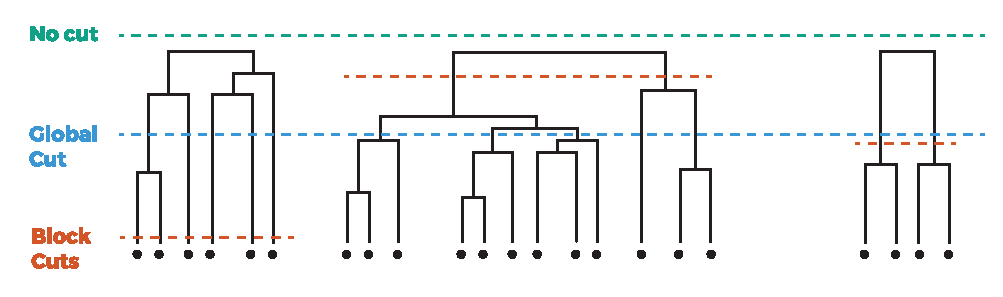
\includegraphics[width=\textwidth]{./figures/fig-cuts.pdf}
\end{figure}

\end{frame}


% Evaluation =====================================================================

\begin{frame}{Evaluation}

{\it Protocol:} Use the {\color{blue} claimed signatures} (about 1M) to form {\color{blue} ground truth clusters}. Keep 10\% as a training set to find model parameters, and 90\% as a test set for evaluation.

\begin{align}
\text{$B^3$ Precision} &= \mathbb{E}_s \{ \frac{|\hat{C}(s) \cap C(s)|}{|\hat{C}(s)|}  \} \\
\text{$B^3$ Recall} &= \mathbb{E}_s \{ \frac{|\hat{C}(s) \cap C(s)|}{|C(s)|}  \} \\
\text{$B^3$ F-score} &= \frac{2 \times \text{Precision} \times \text{Recall}}{\text{Precision} + \text{Recall}}
\end{align}

where $C(s)$ (resp., $\hat{C}(s)$) is the true (resp., predicted) set of signatures to which $s$ belongs.


% disambiguation is clustering
% how to evaluate clustering?
% give number for simple strategy (all same names baseline 0.5, all same block baseline 1.0)
\end{frame}

% Results =====================================================================

\begin{frame}{Results}

\begin{table}
    \centering
    \begin{tabular}{| l c |}
    \hline
        \textit{Method} & \textit{$B^3 \text{F-score}$}  \\
    \hline
    \hline
    Full name & 0.8183 \\
    Last name + First initial & 0.9409 \\
    \hline
    Our model & {\color{blue} 0.9868} \\
    \hline
    \end{tabular}
\end{table}

\end{frame}

% Results =====================================================================

\begin{frame}{Results 1 of 2}

\begin{table}
\caption{Average precision, recall and f-measure scores on test folds. CUnderlined row corresponds to the state-of-the-art choices.}
\centering
\begin{tabular}{|l|c c c |}
  \hline
                       & \multicolumn{3}{|c|}{\textbf{B3}}\\
  \textbf{Description} & $P$ & $R$ & $F$ \\
  \hline
  \hline
Baseline & 0.9024 & 0.9828 & 0.9409  \\
\hline
\underline{Blocking = SFI} & 0.9901 & 0.9760 & 0.9830  \\
Blocking = Double metaphone & 0.9856 & 0.9827 & 0.9841  \\
Blocking = NYSIIS & 0.9875 & 0.9826 & \textbf{0.9850}   \\
Blocking = Soundex & 0.9886 & 0.9745 & 0.9815  \\
\hline
\underline{Classifier = GBRT} & 0.9901 & 0.9760 & 0.9830   \\
Classifier = Random Forests & 0.9909 & 0.9783 & \textbf{0.9846}  \\
Classifier = Linear Regression & 0.9749 & 0.9584 & 0.9666 \\
\hline
Training pairs = Non-blocked, uniform & 0.9793 & 0.9630 & 0.9711   \\
Training pairs = Blocked, uniform & 0.9854 & 0.9720 & 0.9786   \\
\underline{Training pairs = Blocked, balanced} & 0.9901 & 0.9760 & \textbf{0.9830}  \\
\hline

\end{tabular}
\end{table}

\end{frame}

% Results =====================================================================

\begin{frame}{Results 2 of 2}

\begin{table}
\caption{Average precision, recall and f-measure scores on test folds. Underlined row corresponds to the state-of-the-art choices.}
\centering
\begin{tabular}{|l|c c c |}
  \hline
                       & \multicolumn{3}{|c|}{\textbf{B3}}\\
  \textbf{Description} & $P$ & $R$ & $F$ \\
  \hline
  \hline
Baseline & 0.9024 & 0.9828 & 0.9409  \\
\hline
\underline{Clustering = Average linkage} & 0.9901 & 0.9760 & \textbf{0.9830}  \\
Clustering = Single linkage & 0.9741 & 0.9603 & 0.9671  \\
Clustering = Complete linkage & 0.9862 & 0.9709 & 0.9785   \\
\hline
No cut (baseline) & 0.9024 & 0.9828 & 0.9409   \\
Global cut & 0.9892 & 0.9737 & 0.9814   \\
\underline{Block cut} & 0.9901 & 0.9760 & \textbf{0.9830} \\
\hline
\textbf{Combined best settings} & 0.9888 & 0.9848 & \textbf{0.9868}  \\
Best settings without ethnicity features & 0.9862 & 0.9819 & 0.9841 \\
\hline

\end{tabular}
\end{table}

\end{frame}

% Results =====================================================================

\begin{frame}{Summary Results}

\begin{table}
    \centering
    \begin{tabular}{| l c |}
    \hline
        \textit{Method} & \textit{$B^3 \text{F-score}$}  \\
    \hline
    \hline
    Full name & 0.8183 \\
    Last name + First initial & 0.9409 \\
    \hline
    Our model & {\color{blue} 0.9868} \\
    \hline
    \end{tabular}
\end{table}

\end{frame}

% Future Work ================================================================

\begin{frame}{Future Work}

\begin{itemize}
\item Error analysis.\\[2em]

\item Explore Author2Vec approach as a partitioning (blocking) strategy.\\[2em]

\item Build more comprehensive name-ethnicity dataset. \\[2em]

\item Archive and utilize user's feedback to enhance the model \\[2em]

\end{itemize}

\end{frame}


\end{document}
